%% This file was auto-generated by IPython.
%% Conversion from the original notebook file:
%% rndsvd.ipynb
%%
\documentclass[11pt,english,fleqn]{article}

%% This is the automatic preamble used by IPython.  Note that it does *not*
%% include a documentclass declaration, that is added at runtime to the overall
%% document.

\usepackage{amsmath}
\usepackage{amssymb}
\usepackage{graphicx}
\usepackage{ucs}
\usepackage[utf8x]{inputenc}

% needed for markdown enumerations to work
\usepackage{enumerate}

% Slightly bigger margins than the latex defaults
\usepackage{geometry}
\geometry{verbose,tmargin=3cm,bmargin=3cm,lmargin=2.5cm,rmargin=2.5cm}

% Define a few colors for use in code, links and cell shading
\usepackage{color}
\definecolor{orange}{cmyk}{0,0.4,0.8,0.2}
\definecolor{darkorange}{rgb}{.71,0.21,0.01}
\definecolor{darkgreen}{rgb}{.12,.54,.11}
\definecolor{myteal}{rgb}{.26, .44, .56}
\definecolor{gray}{gray}{0.45}
\definecolor{lightgray}{gray}{.95}
\definecolor{mediumgray}{gray}{.8}
\definecolor{inputbackground}{rgb}{.95, .95, .85}
\definecolor{outputbackground}{rgb}{.95, .95, .95}
\definecolor{traceback}{rgb}{1, .95, .95}

% Framed environments for code cells (inputs, outputs, errors, ...).  The
% various uses of \unskip (or not) at the end were fine-tuned by hand, so don't
% randomly change them unless you're sure of the effect it will have.
\usepackage{framed}

% remove extraneous vertical space in boxes
\setlength\fboxsep{0pt}

% codecell is the whole input+output set of blocks that a Code cell can
% generate.

% TODO: unfortunately, it seems that using a framed codecell environment breaks
% the ability of the frames inside of it to be broken across pages.  This
% causes at least the problem of having lots of empty space at the bottom of
% pages as new frames are moved to the next page, and if a single frame is too
% long to fit on a page, will completely stop latex from compiling the
% document.  So unless we figure out a solution to this, we'll have to instead
% leave the codecell env. as empty.  I'm keeping the original codecell
% definition here (a thin vertical bar) for reference, in case we find a
% solution to the page break issue.

%% \newenvironment{codecell}{%
%%     \def\FrameCommand{\color{mediumgray} \vrule width 1pt \hspace{5pt}}%
%%    \MakeFramed{\vspace{-0.5em}}}
%%  {\unskip\endMakeFramed}

% For now, make this a no-op...
\newenvironment{codecell}{}

 \newenvironment{codeinput}{%
   \def\FrameCommand{\colorbox{inputbackground}}%
   \MakeFramed{\advance\hsize-\width \FrameRestore}}
 {\unskip\endMakeFramed}

\newenvironment{codeoutput}{%
   \def\FrameCommand{\colorbox{outputbackground}}%
   \vspace{-1.4em}
   \MakeFramed{\advance\hsize-\width \FrameRestore}}
 {\unskip\medskip\endMakeFramed}

\newenvironment{traceback}{%
   \def\FrameCommand{\colorbox{traceback}}%
   \MakeFramed{\advance\hsize-\width \FrameRestore}}
 {\endMakeFramed}

% Use and configure listings package for nicely formatted code
\usepackage{listingsutf8}
\lstset{
  language=python,
  inputencoding=utf8x,
  extendedchars=\true,
  aboveskip=\smallskipamount,
  belowskip=\smallskipamount,
  xleftmargin=2mm,
  breaklines=true,
  basicstyle=\small \ttfamily,
  showstringspaces=false,
  keywordstyle=\color{blue}\bfseries,
  commentstyle=\color{myteal},
  stringstyle=\color{darkgreen},
  identifierstyle=\color{darkorange},
  columns=fullflexible,  % tighter character kerning, like verb
}

% The hyperref package gives us a pdf with properly built
% internal navigation ('pdf bookmarks' for the table of contents,
% internal cross-reference links, web links for URLs, etc.)
\usepackage{hyperref}
\hypersetup{
  breaklinks=true,  % so long urls are correctly broken across lines
  colorlinks=true,
  urlcolor=blue,
  linkcolor=darkorange,
  citecolor=darkgreen,
  }

% hardcode size of all verbatim environments to be a bit smaller
\makeatletter 
\g@addto@macro\@verbatim\small\topsep=0.5em\partopsep=0pt
\makeatother 

% Prevent overflowing lines due to urls and other hard-to-break entities.
\sloppy

\setlength{\mathindent}{0pt}
\setlength{\parindent}{0pt}
\setlength{\parskip}{8pt}
\begin{document}

\section{Rasgele İzdüşümü (Random Projection) ile SVD}

Bir matrisin rasgele izdusumunu almak, yani onu rasgele bir sayilardan
olusan bir matris ile sagdan carpmak bize ne kazandirir? Elde edilen
yeni matrisin ozellikleri nedir?

Suradaki {[}1{]} arastirmaya gore bu yeni matristeki satirlar (veri
noktalarimiz yani) arasindaki mesafeler fazla degismemektedir. Burada
``fazla'' olarak niteledigimiz {[}1{]}'de daha detayli olarak isleniyor.
Yapay Ogrenim baglaminda rasgele izdusumun bize kazandirdigi en onemli
fayda ana matris $A$ uzerinde boyut kucultme yapabilmemizdir. Diyelim ki
$m \times n$ boyutundaki $A$'yi $n \times k$ boyutunda bir rasgele
matris $\Omega$ ile carptigimiz zaman elde ettigimiz $m \times k$
boyutunda yeni bir matris. Eger $n$ milyarlar boyutunda ise, bizim
tanimladigimiz bir $k$ uzerinden matris boyutunu (kolonlari) 100 ya da
1000'e indirebilmis oluyoruz.

Literaturde hedeflenenin $|| A - \tilde{A} || < \epsilon$

yani A'dan onun yaklasiksal benzeri cikartilinca bu farkin normunun cok
ufak $\epsilon$ olmasinin amaclandigi gorulecektir. $\tilde{A}$'yi elde
etmek icin su mantigi uygulayalim
\[ A = QR \]\[ Q^TA = R \]\[ QQ^TA = QR \]\[ QQ^TA = A \]
Simdi eger $Q$ yaklasiksal olarak bulunmus, ve daha dusuk boyutta ise,
otomatik olarak ustteki $A$ da yaklasiksal olacaktir.

Bunun icin bir rasgele matris yaratilir, bu matrisin her ogesinin bir 0
merkezli 1 standart sapmali Gaussian'dan orneklenebilir, sonra bu matris
$A$ ile carpilir
\[ Y  = A\Omega \]
Ortaya cikan $Y$'nin $A$'nin ``menzilini (range)'' yaklasiksal olarak
temsil ettigi de soylenir, bu mantiklidir, cunku bir matrisin menzilinin
ne oldugunu dusunursek, onun tum kolonlarinin her turlu carpilip
toplanmasinin olusturdugu uzay bu menzildir. Simdi kolonsal carpim
gorusunu kullanirsak, $A$'yi bir baska rasgele matris ile sagdan
carpmak, evet, yaklasiksal olarak onun kolonlarini degisik
kombinasyonlarda, birbirleriyle toplamak anlamina gelecektir, ortaya
cikan yeni matris te $A$'nin menzilini kismen temsil edebilir. Simdi bu
menzilden ``geriye giderek'' onun bazini ortaya cikarabiliriz.
Unutmayalim, yeni matris $A$'nin boyutu azaldi, artik elimizde
$m \times k$ boyutunda bir matris var.
\[ Y = QR \]
ile $Q$ matrisini elde ederiz. Bu guzel bir sonuc. Simdi ustteki
$QQ^TA = A$ ifadesine geri donelim,
\[ \tilde{A} = QQ^TA \]
Eger
\[Q^TA = B\]
dersek,
\[ \tilde{A} \approx QB \]
seklinde yeni bir ayristirma elde ederiz. Ayrica bu $A$'ya yaklasiksal
olarak ulasmanin baska bir yoludur da. Elimide $B$ ve $Q$ var ise (ki
var, cunku $B$ rasgele izdusumden geldi, $Q$ bunun uzerinde $QR$
ayristirmasi sonrasi elde edildi), bu iki matrisin carpimi bize
yaklasiksal $A$'yi verecektir. Bu yaklasiksal $\tilde{A}$ uzerinde SVD
gerceklestirmek te mumkundur. Yeni matrisin boyutlari $k \times n$
olacaktir.

Test olarak IRIS veri seti uzerinde

\begin{codecell}
\begin{codeinput}
\begin{lstlisting}
import numpy.random as rand
import numpy.linalg as lin
import pandas as pd

df = pd.read_csv("iris.csv",sep=',')

A = np.array(df)[:,0:4]

n = 4; k = 3

Omega = rand.randn(n,k)

# Rasgele SVD

Y = np.dot(A, Omega)

Q, R = lin.qr(Y)

B = np.dot(Q.T, A)

Uhat, Sigma, V = lin.svd(B)

U = np.dot(Q, Uhat)

plt.plot(U[:,0],U[:,1],'r+')

plt.hold(True)

# Direk A uzerinde SVD

U, Sigma, V = lin.svd(A);

plt.plot(U[:,0],U[:,1],'bx')

plt.show()

\end{lstlisting}
\end{codeinput}
\begin{codeoutput}
\begin{center}
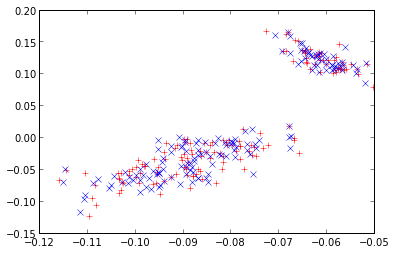
\includegraphics[width=0.7\textwidth]{rndsvd_files/rndsvd_fig_00.png}
\par
\end{center}
\end{codeoutput}
\end{codecell}
Rasgele izdusum sonrasi SVD noktalari kirmizi, direk SVD noktalari mavi
ile gosterildi. 4 boyutu 3 boyuta izdusum yaptik, ve ardindan ek bazi
operasyonlar sonrasi SVD aldik. Sonuc goruldugu gibi oldukca birbirine
yakin.

Kaynaklar

{[}1{]} Halko, N., Randomized methods for computing low-rank
approximations of matrices

{[}2{]} Gupta, A., Dasgupta, S., An Elementary Proof of a Theorem of
Johnson and Lindenstrauss

\end{document}
